\documentclass[../../main.tex]{subfiles}
% \graphicspath{{\subfix{../images/}}}

\begin{document}
\subsection{¿Qué es una Evaluación de Impacto?}
\begin{comment}
El uso de métodos cuantitativos para medir el impacto de programas sociales ha cobrado un gran interés en los últimos años \cite{bernal}. Las evaluaciones de impacto han comenzado a desempeñar un papel preponderante en el diseño de políticas públicas \cite{bernal}.
\end{comment}

Los programas y políticas de desarrollo suelen estar diseñados para cambiar resultados, como aumentar los ingresos, mejorar el aprendizaje o reducir las enfermedades \cite{gertler-2016}. Saber si estos cambios se logran o no es una pregunta crucial para las políticas públicas \cite{gertler-2016}, y el método para responderla es lo que se conoce como \textbf{evaluación de impacto}.

Una evaluación de impacto mide los cambios en el bienestar de los individuos que se pueden atribuir a un proyecto, un programa o una política específicos \cite{gertler-2016}. Su sello distintivo radica en que pueden proporcionar \textbf{evidencia} robusta y creíble sobre si un programa concreto ha alcanzado o está alcanzando sus objetivos \cite{gertler-2016}. 

Estas evaluaciones ponen un fuerte énfasis en los resultados y buscan responder una pregunta específica de causa y efecto: ¿cuál es el impacto (o efecto causal) de un programa? Más precisamente, intentan identificar  y cuantificar los cambios directamente atribuibles al tratamiento \cite{gertler-2016} sobre un conjunto de \textbf{variables de resultado} o \textbf{de interés} en un conjunto de individuos \cite{bernal}. Estas variables son aquellas sobre las cuales se espera que el programa tenga un efecto en los beneficiarios \cite{bernal}. Podrían ser por ejemplo la estatura y peso de los individuos, la cantidad de empleados o de ventas en una empresa, o indicadores de salud de un paciente.

Por lo tanto, el objetivo final de la evaluación de impacto consiste en establecer lo que se conoce como \textbf{efecto del tratamiento}, que es la diferencia entre la variable de resultado del individuo participante en el programa en presencia del programa, y la variable de resultado de ese individuo en ausencia del programa \cite{bernal}. Sin embargo, es evidente que la respuesta a qué habría pasado con los beneficiarios si no hubieran recibido el tratamiento se refiere a una situación que no es observable. Este resultado hipotético se denomina \textbf{contrafactual} y es lo que se debe estimar en cualquier evaluación de impacto.

Algunas de las principales razones por las que se debería promover el uso de estas evaluaciones como herramientas de gestión provienen del hecho que permiten mejorar la rendición de cuentas, la inversión de recursos públicos o la efectividad de una política, obtener financiamiento, como así también probar modalidades de programas alternativos o innovaciones de diseño \cite{gertler-2016} y revelar la realidad de muchas políticas públicas para de esta forma contribuir a la fiscalización mediática \cite{bernal}.

Un ejemplo claro de por qué son necesarias las evaluaciones de impacto es el que describe Howard White con respecto al Programa Integrado de Nutrición en Bangladesh (PINB) \cite{white2009theory}. Este programa identificaba, mediante mediciones en campo, a los niños desnutridos y los asignaba a un tratamiento que incluía alimentación suplementaria a los menores y educación nutricional a las madres \cite{bernal}. Inicialmente, el programa fue considerado como un éxito ya que los datos de monitoreo mostraban caídas importantes en los niveles de desnutrición. El Banco Mundial decidió, con base en esta evidencia y previo a cualquier tipo de evaluación, aumentar los recursos destinados al programa. Sin embargo, las primeras evaluaciones de impacto, realizadas por el Grupo Independiente de Evaluación del mismo Banco Mundial y por la ONG inglesa \textit{Save the Children}, mostraron que la mejoría de los indicadores de los beneficiarios era similar o inferior a la de otros niños con características comparables que no hacían parte del programa \cite{bernal}. Estos resultados reflejaron que las percepciones de los administradores del programa y de las entidades financiadoras eran erradas, y sugirieron algunos correctivos al programa \cite{bernal}.

\begin{comment}
    AGREGAR EL EJEMPLO DE MEXICO QUE APARECE EN EL GERTLER
\end{comment}

\subsection{Estimación del Tratamiento}
El marco teórico estándar para formalizar el problema de la evaluación de impacto se basa en el \textbf{modelo de resultados potenciales} o \textbf{modelo causal de Rubin} \cite{rubin1974}. 

Formalmente, se definen dos elementos para cada individuo \(i = 1,...,N\), donde \(N\) denota la población total:
\begin{itemize}
    \item Por un lado, el indicador de tratamiento \(D_i\), tal que \(D_i = 1\) implica que el individuo \(i\) participó del tratamiento, y \(D_i = 0\) en caso contrario.
    \item Por otro lado, las variables de resultado las definimos como \(Y_i(D_i) = Y_i|D_i\) - se lee como ``el valor de \(Y_i\) \textit{dado} \(D_i\)''. De esta forma, \(Y_i(1)\) es la variable de resultado si el individuo \(i\) es tratado, e \(Y_i(0)\) es la variable de resultado si el individuo \(i\) no es tratado. Estos valores son los resultados potenciales.
\end{itemize}

Con esto, el \textbf{efecto del tratamiento} para un individuo \(i\) se puede escribir como:
\begin{equation}
    \tau_i = Y_i(1) - Y_i(0) = (Y_i|D_i=1) - (Y_i|D_i=0)
    \label{eq:ite} % ite = individual treatment effect
\end{equation}

Según esta fórmula, el impacto causal (\(\tau\)) de un programa (\(D\)) en una variable de resultado (\(Y\)) para un individuo \(i\) es la diferencia entre la variable con el programa (\(Y_i(1)\)) y la misma variable sin el programa (\(Y_i(0)\)). 

De nuevo, el problema fundamental de la evaluación de impacto es que se intenta medir una variable en un mismo momento del tiempo para la misma unidad de observación pero en dos realidades diferentes. Sin embargo, claramente solo se da uno de los dos resultados potenciales \(Y_i(1)\) o \(Y_i(0)\), pero no ambos. Es decir, en los datos queda solamente registrado \(Y_i(1)\) si \(D_i=1\) e \(Y_i(0)\) si \(D_i=0\); no se dispone de \(Y_i(1)\) si el individuo no fue tratado (\(D_i=0\)), ni tampoco de \(Y_i(0)\) si el individuo fue tratado (\(D_i=1\)). De esta manera, el \textbf{resultado observado de \(Y_i\)} se puede expresar como:
\begin{equation}
    Y_i = D_i Y_i(1) + (1-D_i)Y_i(0) =
    \begin{cases}
        Y_i(1) \text{ si } D_i=1 \\
        Y_i(0) \text{ si } D_i=0
    \end{cases}
    \label{eq:observed-result}
\end{equation}

Si nos concentramos en las unidades tratadas, en la Ecuación \ref{eq:ite}, el término \(Y_i(0) = (Y_i|D_i=0)\) representa la situación contrafactual, es decir \textit{cuál habría sido el resultado si la unidad no hubiera participado en el programa}. Al ser imposible observar directamente el contrafactual, es necesario \textbf{estimarlo}. La forma más directa de solucionar este problema sería hallando un ``clon perfecto'' para cada uno de los individuos participantes del programa pero que no haya participado, lo cual resulta bastante difícil. Por lo tanto, el primer paso para lograr esta estimación consiste en \textbf{desplazarse desde el nivel individual al nivel del grupo} \cite{gertler-2016}, concentrando el análisis en el \textbf{impacto} o \textbf{efecto \textit{promedio}} (y no individual).

En primera instancia, se puede estimar el \textbf{impacto promedio del programa \textit{sobre la población}} (o \(ATE\), del inglés \textit{Average Treatment Effect}):
\begin{equation}
    ATE = \mathbb{E}\left[Y_i(1)-Y_i(0)\right]
\end{equation}
donde el operador \(\mathbb{E}\) representa la media de una variable aleatoria.

El \(ATE\) se interpreta como el cambio promedio en la variable de resultado cuando un individuo escogido al azar pasa aleatoriamente de ser participante a ser no participante \cite{bernal}, es decir representa el efecto esperado del tratamiento si toda la población fuera tratada. Esta medida es relevante en el caso de la evaluación de un programa universal. Es importante notar que para calcularlo, habría que estimar un contrafactual tanto para los tratados como para los no tratados.

Sin embargo, en la mayoría de los casos, el tratamiento solo está disponible para un subconjunto de la población, ya sea por restricciones presupuestarias o criterios de elegibilidad, entre otras razones. Además, también ocurre que no todos los que fueron seleccionados para recibirlo efectivamente participan o se inscriben. En estos casos, suele ser más relevante estimar el efecto únicamente en quienes efectivamente recibieron el tratamiento.

Por lo tanto, se define el \textbf{impacto promedio del programa \textit{sobre los tratados}} (o \(ATT\), del inglés \textit{Average Treatment Effect on the Treated}), que es en general el parámetro de mayor interés en una evaluación de impacto, y representa el efecto esperado del tratamiento en el subconjunto de individuos que fueron efectivamente tratados:
\begin{equation}
    ATT = \mathbb{E} \left[Y_i(1)-Y_i(0)|D_i=1\right] = \mathbb{E} \left[Y_i(1)|D_i=1\right] - \mathbb{E} \left[Y_i(0)|D_i=1\right]
    \label{eq:ATT}
\end{equation}
Es decir, el \(ATT\) es la diferencia entre la media de la variable de resultado en el grupo de los participantes y la media que hubieran obtenido los participantes si el programa no hubiera existido \cite{bernal}.

\subsection{El Grupo de Control como Estimador del Contrafactual}
En la ecuación \ref{eq:ATT}, el término \(\mathbb{E} \left[Y_i(1)|D_i=1\right]\) es un resultado observable mientras que \(\mathbb{E} \left[Y_i(0)|D_i=1\right]\) es el promedio contrafactual que debemos aproximar. Para lograrlo, se construye lo que se conoce como \textbf{grupo de control} o \textbf{de comparación}, formado por individuos que no participan del programa pero que, idealmente, son estadísticamente similares \cite{gertler-2016} al \textbf{grupo de tratamiento}, compuesto por quienes sí recibieron el programa. La Figura \ref{fig:control-group} ilustra esta distinción. A partir de ahora, denotaremos con \(C_i\) a un individuo \(i\) que pertenezca al grupo de control.

\begin{figure}[h!]
    \centering
    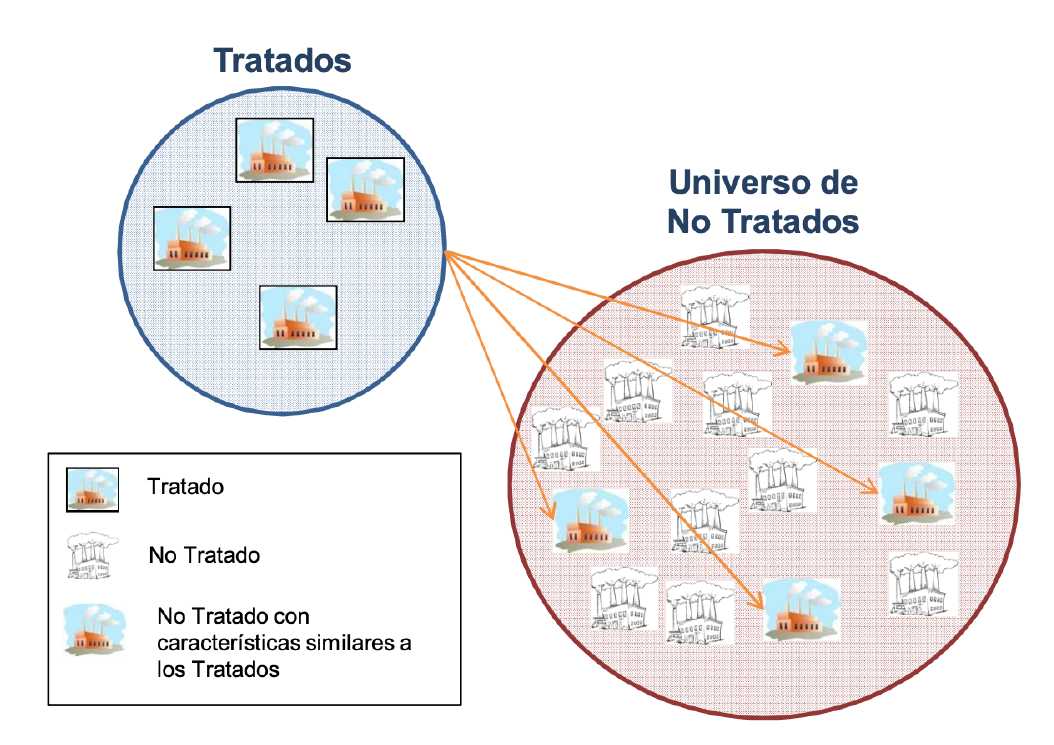
\includegraphics[width=0.65\textwidth]{figs/grupo-de-control.png}
    \caption{El grupo de control debería estar formado idealmente por individuos que no recibieron el tratamiento pero que en promedio poseen características similares a los tratados.}
    \label{fig:control-group}
\end{figure}

Por lo tanto, en la práctica, el reto está en definir un \textit{buen} grupo de control, es decir uno que sea estadísticamente idéntico al de tratamiento, en promedio, en ausencia del programa \cite{gertler-2016}. Si se lograra que los dos grupos sean idénticos, con la única excepción que un grupo participa del programa y el otro no, entonces sería posible estar seguros que cualquier diferencia en los resultados tiene que deberse al programa \cite{gertler-2016}.

Para que un grupo de comparación sea válido, debe satisfacer lo siguiente \cite{gertler-2016}:
\begin{itemize}
    \item Las características \textit{promedio} del grupo de tratamiento y del grupo de comparación deben ser idénticas en ausencia del programa. Cabe resaltar que no es necesario que las unidades individuales en el grupo de tratamiento tengan clones perfectos en el grupo de control.
    \item No debe ser afectado por el tratamiento de forma directa ni indirecta.
    \item El grupo de comparación debería reaccionar de la misma manera que el grupo de tratamiento si fuera objeto del programa.
\end{itemize}

Cuando el grupo de comparación no produce una estimación precisa del contrafactual, no se puede establecer el verdadero impacto del programa. A continuación, se presentan dos situaciones en las que esto ocurre.

\subsubsection{Comparaciones antes-después}
Este tipo de comparaciones intenta establecer el impacto de un programa a partir de un seguimiento de los cambios en los resultados en los participantes del programa a lo largo del tiempo. Consideran el contrafactual como el resultado para el grupo de tratamiento antes que comience la intervención, momento también conocido como \textbf{línea de base}. Esta comparación supone que si el programa no hubiera existido, el resultado para los participantes del programa habría sido igual a su situación antes del programa, lo cual en la mayoría de los tratamientos este supuesto no puede sostenerse \cite{gertler-2016}.

\subsubsection{Comparaciones de inscritos y no inscritos: Sesgo de autoselección}
Como explicamos anteriormente, el término \(\mathbb{E} \left[Y_i(0)|D_i=1\right]\) de la Ecuación \ref{eq:ATT} representa el contrafactual, que no es observable. Sin embargo, lo que sí se puede medir es la variable de resultado entre los no inscritos, aquellos individuos que no participaron del programa, es decir \(\mathbb{E} \left[Y_i(0)|D_i=0\right]\).

Por lo tanto, podríamos tomar a todo el conjunto de los no participantes como grupo de control y solucionar el problema del contrafactual utilizando \(\mathbb{E} \left[Y_i(0)|D_i=0\right]\) como estimador, es decir podríamos asumir lo siguiente:  
\begin{equation}
    \mathbb{E} \left[Y_i(0)|D_i=1\right]\ = \mathbb{E} \left[Y_i(0)|D_i=0\right]\
    \label{eq:supuesto-IC}  % IC: Independencia Condicional
\end{equation}
Esto quiere decir que el valor esperado de la variable de resultado en ausencia del programa (\(\mathbb{E}\left[Y_i(0)\right]\)) es idéntico para el grupo de tratados (\(D = 1\)) y para el de no tratados (\(D = 0\)), lo que se conoce como el \textbf{supuesto de Independencia Condicional}. Indica que los individuos que participan en el programa no son sistemáticamente distintos de los que no lo hacen \cite{bernal} o, en otras palabras, que la decisión de participar en el programa no está determinada por factores que también influyen en la variable de resultado.

De esta forma, podríamos calcular el \(ATT\) como:
\begin{equation}
    ATT = \mathbb{E} \left[Y_i(1)|D_i=1\right] - \mathbb{E} \left[Y_i(0)|D_i=0\right]
    \label{eq:ATT-con-supuesto-IC}
\end{equation}

Sin embargo, el supuesto de Independencia Condicional se viola toda vez que la participación en el programa es una \textit{elección} del individuo elegible \cite{bernal}. La razón es que los participantes y los no participantes generalmente son diferentes, aún en ausencia del programa, y son justamente esas diferencias que llevan a que algunos individuos escojan participar y otros no. Por lo tanto, si en estos casos se toma como grupo de control a todos aquellos que no decidieron participar y se mide el impacto con respecto a ellos, puede ocurrir que la diferencia en los resultados se deba a características propias de los individuos que llevaron a unos a anotarse y a otros no.

Este problema se conoce como \textbf{sesgo de autoselección}, ya que los integrantes del grupo de control se \textit{autoseleccionaron} para no participar del programa. Más concretamente, este sesgo se produce cuando los motivos por los que un individuo participa en un programa, usualmente no observables y difíciles de medir, están correlacionados con los resultados \cite{gertler-2016}, y por ende, es muy probable que la variable de resultado del grupo de tratamiento y del grupo de control sean diferentes, \textit{aún si el programa no existiera} \cite{bernal}. Intuitivamente, si hay variables que explican tanto la participación como la variable de resultado, la comparación de medias puede estar atribuyendo al programa un efecto que en realidad se debe a las diferencias preexistentes entre el grupo de tratamiento y el grupo de control \cite{bernal}.

Un buen ejemplo de esta situación lo presenta \cite{bernal}, en el que se plantea un programa de nutrición infantil. Podría ocurrir que las madres de familias participantes del programa sean más proactivas respecto al desarrollo de sus hijos, por lo cual se preocuparon en lograr la participación en el programa. El problema de autoselección en este caso radica en que la motivación de las madres (que no se observa y es difícil de medir) afecta no solo la probabilidad de participar en el programa, sino también el estado nutricional de los niños ya que estas podrían vigilar mejor la dieta de sus hijos. De esta forma, la diferencia observada en el estado nutricional de los niños de los dos grupos podría deberse parcialmente a la diferencia en el nivel de compromiso de las madres, y no exclusivamente a que un grupo participa en el programa y el otro no.

Podemos plantear este problema más formalmente. Notemos que podemos reescribir la fórmula del \(ATT\) (\ref{eq:ATT}) de la siguiente manera:
\begin{equation}
    ATT + \mathbb{E} \left[Y_i(0)|D_i=1\right] = \mathbb{E} \left[Y_i(1)|D_i=1\right] 
    \label{eq:ATT2}
\end{equation}
Si ahora restamos \(\mathbb{E} \left[Y_i(0)|D_i=0\right]\) a ambos lados, obtenemos:
\begin{equation}
    \mathbb{E} \left[Y_i(1)|D_i=1\right] - \mathbb{E} \left[Y_i(0)|D_i=0\right]\ = ATT + \mathbb{E} \left[Y_i(0)|D_i=1\right] - \mathbb{E} \left[Y_i(0)|D_i=0\right]\
    \label{eq:ATT3}
\end{equation}

De esta forma, el sesgo de autoselección aparece en el término \(\mathbb{E} \left[Y_i(0)|D_i=1\right] - \mathbb{E} \left[Y_i(0)|D_i=0\right]\).

Dicho esto, el gran desafío de la evaluación de impacto es determinar las condiciones o supuestos bajo los cuales \(\mathbb{E} \left[Y_i(0)|D_i=0\right]\) se puede utilizar como una estimación válida del contrafactual \(\mathbb{E} \left[Y_i(0)|D_i=1\right]\) \cite{bernal}, y por lo tanto utilizarse para poder aproximar el valor del \(ATT\). Asegurarse de que el impacto estimado esté libre de sesgo de autoselección es uno de los principales objetivos de cualquier evaluación
de impacto, y plantea importantes dificultades \cite{gertler-2016}. 

\begin{comment}
\bigskip
Es importante en este punto identificar claramente los diferentes resultados que hemos mencionado hasta el momento, los cuales se encuentran en la Tabla \ref{tab:distinciones}.
\begin{table}[h!]
    \centering
    \begin{tabular}{p{7cm}m{7cm}}  % Set fixed column widths
        \hline
        \textbf{Lo que se desea medir}: el \(ATT\). & \(\mathbb{E} \left[Y_i(1)-Y_i(0)|D_i=1\right]\) \\
        \hline
        \textbf{Lo que se observa}: el promedio de la diferencia entre los resultados de los tratados y el grupo de control. & \(\mathbb{E} \left[Y_i(1)-C_i(0)\right]\) \\
        \hline
        \textbf{El sesgo de autselección}: el promedio de la diferencia potencial entre lo que se observa y lo que se desea medir. & \(\mathbb{E} \left[\left(Y_i(1)-Y_i(0)\right) - \left(Y_i(1)-C_i(0)\right)\right] = \mathbb{E} \left[C_i(0)-Y_i(0)\right]\) \\
        \hline
    \end{tabular}
    \caption{Distinción entre las diferentes comparaciones presentes en una evaluación de impacto.}
    \label{tab:distinciones}
\end{table}
Teniendo en cuenta las fórmulas expuestas en esta tabla, podemos enunciar de otra forma lo que dijimos anteriormente: la calidad de una evaluación de impacto dependerá de los supuestos necesarios para asegurar que no hay sesgo de selección, es decir que \(\mathbb{E} \left[C_i(0)-Y_i(0)\right] = 0\).
\end{comment}

% Los distintos tipos de experimentos?
\bigskip
Las reglas de un programa para seleccionar a los participantes, también llamadas \textbf{reglas de asignación}, constituyen el parámetro clave para determinar el método de evaluación de impacto. A continuación, presentamos las distintas reglas y los métodos de evaluación que se utilizan en la práctica al trabajar con cada una de ellas.

\subsection{Evaluaciones Experimentales o Aleatorias}
En este tipo de evaluaciones, los beneficiarios del programa en cuestión son seleccionados al azar, es decir mediante un sorteo. La asignación aleatoria se considera la regla de oro de la evaluación de impacto ya que no solo proporciona a los administradores del programa una regla imparcial y transparente para asignar recursos escasos entre poblaciones igualmente merecedoras de ellos, sino que también representa el método más sólido para evaluar el impacto de un programa \cite{gertler-2016}.

La asignación aletoria trae dos consecuencias importantes: las unidades ya no pueden \textit{elegir} si participar o no, y además todas tienen la misma probabilidad de ser seleccionadas para el programa. De esta forma, el resultado potencial de cada individuo es independiente de sus condiciones previas, ya que la asignación al tratamiento no está determinada por sus características, sino por el azar.

Como explicamos anteriormente, el grupo de comparación ideal sería lo más similar posible al grupo de tratamiento en todos los sentidos, excepto con respecto a su participación en el programa que se evalúa. Ahora bien, el proceso de asignación aleatoria producirá dos grupos que tienen una alta probabilidad de ser estadísticamente idénticos en todas sus características (observables y no observables), siempre que el número de unidades sea suficientemente grande \cite{gertler-2016}. Esto es así ya que en general, si la población de unidades elegibles es lo suficientemente grande, este mecanismo asegura que cualquier rasgo de la población se transfiere a ambos grupos. Sin embargo, en la práctica, este supuesto debería comprobarse empíricamente con los datos de línea de base de ambos grupos.

Dicho esto, lo que ocurre en estos casos es que todos aquellos individuos que no resultaron ser beneficiarios del programa conforman un grupo de control que resulta ser naturalmente un excelente estimador del contrafactual \(\mathbb{E} \left[Y_i(0)|D_i=1\right]\). Es decir, mediante este tipo de asignación, se asegura que se cumple el supuesto de Independencia Condicional, dado por la ecuación \ref{eq:supuesto-IC}.

La asignación aleatoria puede utilizarse como regla de asignación de un programa en dos escenarios específicos: cuando la población elegible es mayor que el número de plazas disponibles del programa, o  cuando sea necesario ampliar un programa de manera progresiva hasta que cubra a toda la población elegible \cite{gertler-2016}. Además, la asignación aleatoria podría hacerse a nivel individual (por ejemplo, a nivel de hogares), o a nivel de conglomerado (por ejemplo, comunidades) \cite{bernal}.

Una vez que se haya asignado el tratamiento de manera aleatoria, gracias a \ref{eq:supuesto-IC}, es bastante sencillo estimar el impacto del programa. Después de que el programa ha funcionado durante un tiempo, tendrán que medirse los resultados de las unidades de tratamiento y de comparación. El impacto del programa es sencillamente la diferencia entre el resultado promedio para el grupo de tratamiento y el resultado promedio para el grupo de comparación, es decir:
\[
\mathbb{E} \left[Y_i(1)|D_i=1\right]\ - \mathbb{E} \left[Y_i(0)|D_i=0\right]\
\]

Resulta claro que las evaluaciones experimentales tienen varias ventajas: por diseño, resuelven el problema del sesgo de selección, y además los resultados obtenidos son transparentes, intuitivos y no es necesario utilizar herramientas econométricas sofisticadas para alcanzarlos \cite{bernal}. Esto hace que contribuyan a la transparencia de las políticas públicas y a la rendición de cuentas \cite{bernal}.

Sin embargo, este tipo de evaluaciones sufre varias limitaciones que hace que no sea tan común en la práctica. Por un lado, pueden ser costosas y de difícil implementación \cite{bernal}. Esto se debe a que en general, el experimento aleatorio se hace específicamente para evaluar una intervención, por lo que es necesario destinar recursos para la prueba piloto, la recolección de información, los seguimientos, y a veces incluso la implementación del programa \cite{bernal}. Otro problema que tienen, y probablemente el más importante, es que por pertenecer al grupo de control, se \textit{excluye} a un segmento de la población, igualmente vulnerable y elegible, de los beneficios de la intervención \cite{bernal}. Además, dada la imposibilidad de negar los beneficios a un grupo de control por largos períodos, con frecuencia es imposible estimar los impacto de largo lazo \cite{bernal}.   

\subsection{Evaluaciones Cuasi-experimentales}
Las evaluaciones cuasi-experimentales son aquellas que buscan estimar el impacto causal, pero se diferencian de las experimentales en el sentido que no se basan en la asignación aleatoria de la intervención \cite{gertler-2016}, debido a que realizarla no es posible o no es ético. En estos casos, la regla de asignación suele ser menos clara, por lo que se considera una incógnita más en la evaluación, acerca de la cual se deben formular supuestos \cite{gertler-2016}.

Las técnicas cuasi-experimentales intentan \textit{simular} un diseño experimental intentando controlar las diferencias entre los individuos tratados y no tratados bajo diferentes supuestos.

Si bien los métodos cuasi-experimentales pueden ser más adecuados en algunos contextos operativos, requieren más supuestos para garantizar que el grupo de comparación provea una estimación válida del contrafactual, como veremos a continuación al profundizar en algunos de ellos.

\subsubsection{Diferencias en Diferencias}
El modelo de diferencias-en-diferencias (DED) es una manera de controlar la estimación del impacto por las diferencias preexistentes entre el grupo de tratamiento y el de control, que estará formado por todos aquellos individuos elegibles que no recibieron el tratamiento. Es decir, el DED no propone una forma de construir el grupo de control sino una para tener en cuenta las diferencias entre los participantes y no participantes. A grandes rasgos, combina las comparaciones antes-después con las comparaciones de inscritos y no inscritos. 

Este modelo es simplemente el cambio esperado en la variable de resultado \(Y\) entre el período posterior y el período anterior a la implementación del tratamiento en el grupo de tratamiento, menos la diferencia esperada en \(Y\) en el grupo de control en el mismo período \cite{bernal}. Es decir, compara los cambios en los resultados a lo largo del tiempo entre unidades participantes y no participantes. 

Si denotamos con \(Y_1\) al valor de la variable \(Y\) en la línea de base, es decir justo antes de la implementación del programa, y con \(Y_2\) al valor de la misma variable en una período posterior a la implementación (también llamado período de seguimiento), entonces el impacto del programa por el método de DED estaría dado por:
\begin{equation}
    \tau_{DED} = 
        \left(
            \mathbb{E}\left[Y_2|D=1\right] - \mathbb{E}\left[Y_1|D=1\right]
        \right) -
        \left(
            \mathbb{E}\left[Y_2|D=0\right] - \mathbb{E}\left[Y_1|D=0\right]
        \right)
\end{equation}

La diferencia en los resultados antes-después para el grupo inscrito controla por factores que son constantes a lo largo del tiempo en ese grupo, puesto que se está comparando el propio grupo consigo mismo. Sin embargo, todavía quedan los factores externos variables en el tiempo en este grupo. La manera que propone el DID de capturar esos factores es medir el cambio antes-después en los resultados de un grupo que no se recibió el programa pero que estuvo expuesto al mismo conjunto de condiciones ambientales (la segunda diferencia). Si se ``limpia'' la primera diferencia de otros factores variables en el tiempo que influyen en el resultado de interés sustrayendo la segunda diferencia, se habrá eliminado una fuente de sesgo \cite{gertler-2016}.

Es importante señalar que el contrafactual que se estima en este caso es el cambio en los resultados del grupo de tratamiento, y su estimación se logra midiendo el cambio en los resultados del grupo de comparación \cite{gertler-2016}. En lugar de contrastar los resultados entre los grupos de tratamiento y comparación después de la intervención, la técnica de DED estudia las tendencias entre los grupos de tratamiento y comparación \cite{gertler-2016}.

% AGREGAR UN EJEMPLO



\subsubsection{Efectos Fijos}

\subsubsection{Propensity Score Matching}
\begin{comment}
    ESQUEMA:
      1 - Se propone controlar por un vector de variables observables X. Explicar en este punto que para esto sirva y tenga sentido, la decisión  de participación en el programa se tiene que deber SOLAMENTE a las características presentes en X (supuesto de Independencia Condicional)
      2 - Problema de 1: la cantidad de características puede hacerse muy grande.
      3 - Presentar el propensity score o probabilidad de participación.
      4 - Hablar sobre el supuesto de Soporte Común.
      
      ... - Presentar ventajas y desventajas.
\end{comment}



\end{document}